\documentclass[border=10pt]{standalone}
\usepackage{pgfplots}
\pgfplotsset{compat=1.18}
\begin{document}
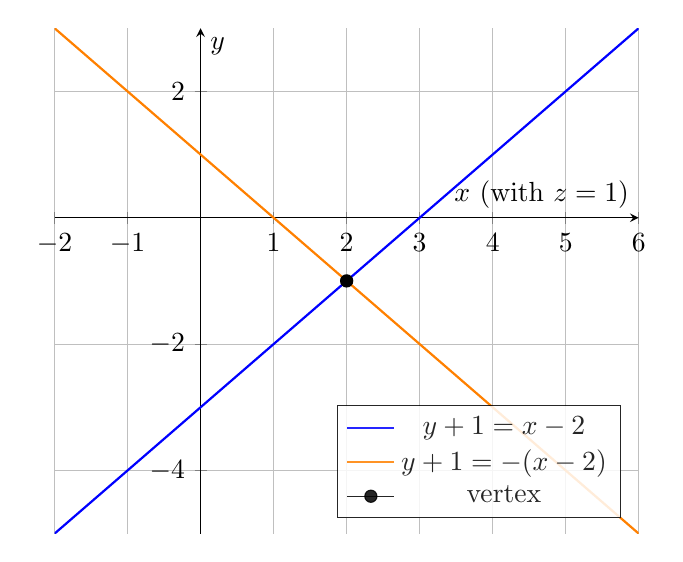
\begin{tikzpicture}
\begin{axis}[
  width=9cm,
  height=8cm,
  axis lines=middle,
  xlabel={$x$ (with $z=1$)},
  ylabel={$y$},
  grid=major,
  xmin=-2, xmax=6,
  ymin=-5, ymax=3,
  legend pos=south east,
  legend style={fill=white, opacity=0.85}
]
\addplot[blue, thick, domain=-2:6, samples=2] {x-3};
\addlegendentry{$y+1=x-2$}
\addplot[orange, thick, domain=-2:6, samples=2] {-x+1};
\addlegendentry{$y+1=-(x-2)$}
\addplot[black, mark=*, mark size=2.2pt] coordinates {(2,-1)};
\addlegendentry{vertex}
\end{axis}
\end{tikzpicture}
\end{document}
